%%%%%%%%%%%%%%%%%%%%%%%%%%%%%%%%%%%%%%%%%%%%%%%%%%%%%%%%%%%%%%%%%%%%%%%%%%%%%%%%%%%%%%%%%%%%%%%%%%%%

\chapter{\ngc253}
\chaptermark{\ngc253}
\label{introduction: chapter: NGC253}

%%%%%%%%%%%%%%%%%%%%%%%%%%%%%%%%%%%%%%%%%%%%%%%%%%%%%%%%%%%%%%%%%%%%%%%%%%%%%%%%%%%%%%%%%%%%%%%%%%%%

\vspace{-0.5cm}
\begin{figure*}[h]
	\centering
	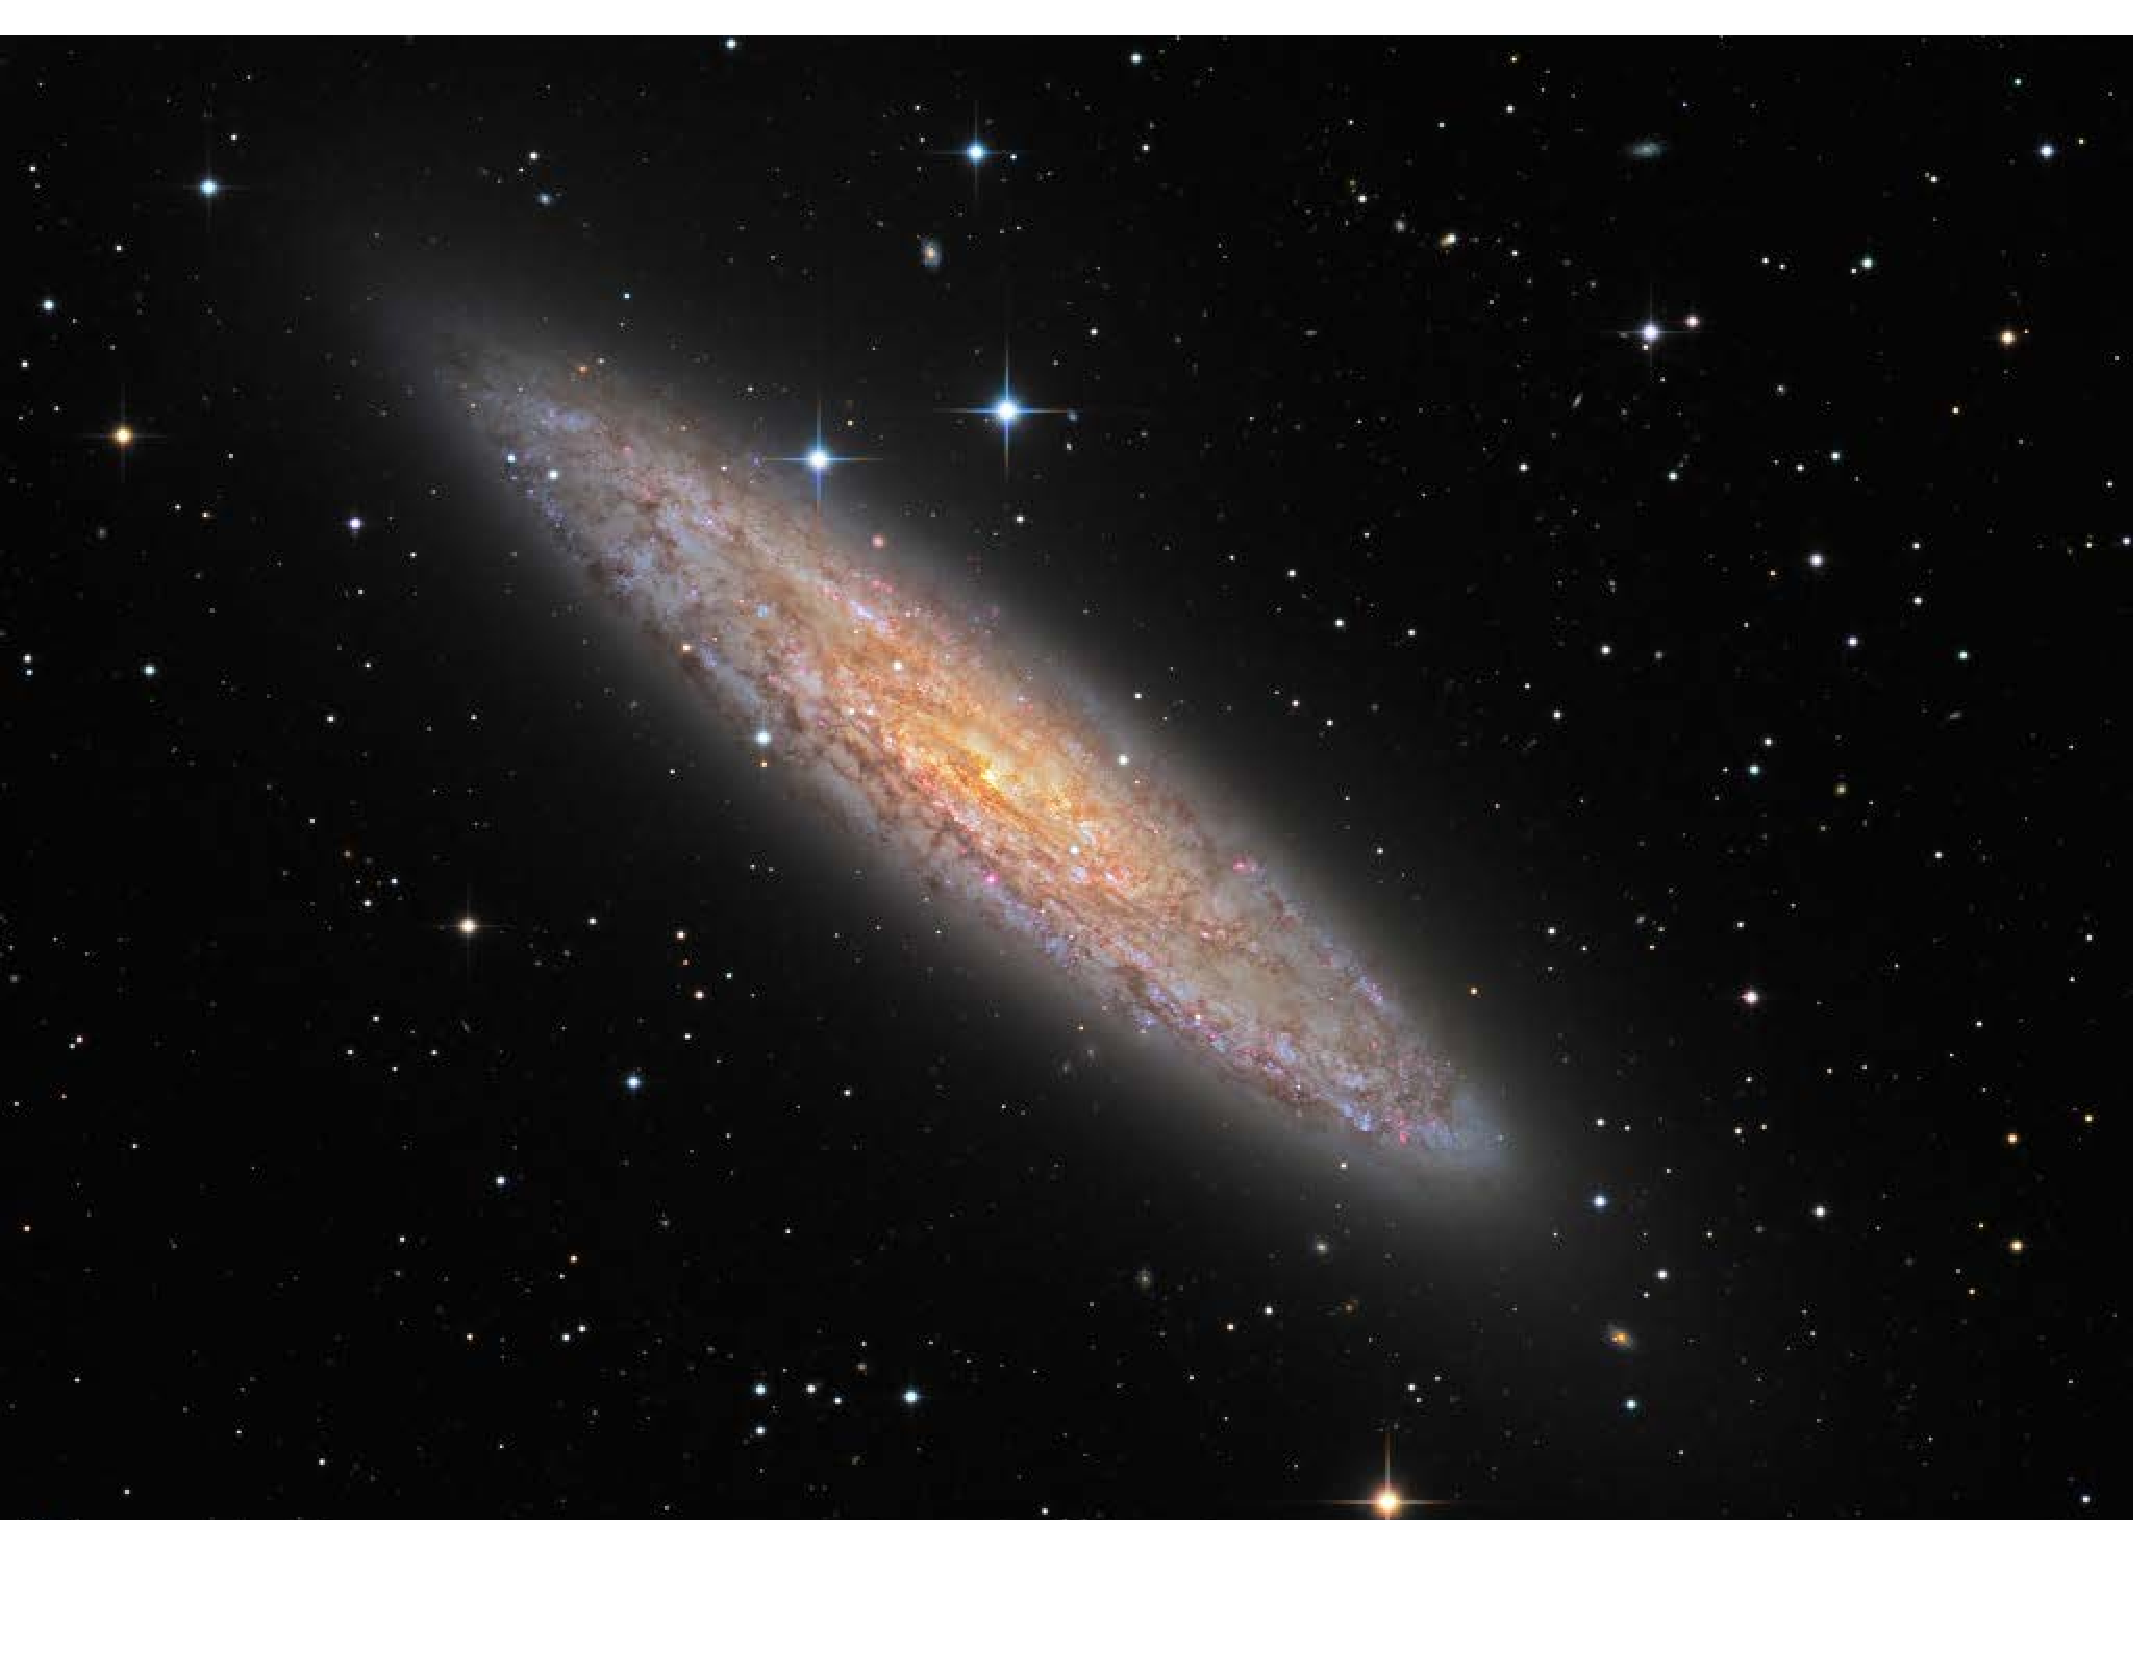
\includegraphics[width=\linewidth]{images/chapters/introduction/ngc253/NGC253_Apod.pdf}
	\caption[Optical image of NGC253]{Optical image of \ngc253. Due to its brightness ($V \sim 7.3$\,mag) and size on the sky ($\sim 30\arcmin$), \ngc253 is a popular target for amateur astronomers who achieve impressive results with extremely long exposure times, 20\,h in this case. Image from \href{https://apod.nasa.gov/apod/ap161103.html}{APOD}, credit: D. Hager, E. Benson}
	\label{introduction: figure: NGC253: optical}
\end{figure*}

\ngc253 is the brightest ($V=7.3$\,mag) galaxy in the Sculptor group, one of the nearest galaxy groups to the local group \citep{2005AJ....129..178K}.
It is also referred to as the Sculptor galaxy or the Silver Coin Galaxy and classified as a barred spiral galaxy (Hubble type SBc).
The stellar mass $M_\ast \sim 4.4 \times 10^{10}$\,\Msun \citep{2011ApJ...736...24B} and total gas mass $M_\mathrm{gas} > 1.3 \times 10^9$\,\Msun \citep{2000PASJ...52..785S}\footnote{Their observations only covered the inner $R<4$\,kpc but not the whole galactic disk.} make \ngc253 a typical L$^\ast$ galaxy, similar to the Milky Way.
Our view on \ngc253 is close to edge-on (inclination $i\sim78^\circ$) and from below the galactic disk.

Due to its proximity, \ngc253 (Figure~\ref{introduction: figure: NGC253: optical}) is an ideal target for high-resolution studies of the physics and chemistry of the star-forming molecular gas and stellar feedback in starbursts.
At a distance of 3.5\,Mpc \citep{Rekola:2005ha}, \ngc253 is one of the nearest starburst systems and considered one of the prototypical starburst galaxies. The star formation rate surface density is $\Sigma_{SFR} \sim 10^2$\,\Msun\,yr$^{-1}$\,kpc$^{-2}$ in the nuclear region which causes the molecular gas depletion time $\tau^\mathrm{mol}_\mathrm{dep}$ to be $\sim 5-25$ times lower than what is found in local disks \citep{Leroy:2015ds}. 
A galactic wind emerges from the central $\sim 200$\,pc of \ngc253 (Figure~\ref{introduction: figure: NGC253: Strickland}) that has been characterized in H$\alpha$, X-ray, as well as neutral and molecular gas emission \citep[e.g.][]{Sharp:2010jl,Turner:1985iy,Sturm:2011jb,Strickland:2000wd,Strickland:2002kp, Westmoquette:2011bp,2000ApJS..129..493H,2013Natur.499..450B,2017ApJ...835..265W}.
The outflow is thought to be stratified with an inner ionized cone and surrounding shells of neutral and molecular gas \citep[as shown in Figure~\ref{introduction: figure: star formation: outflow cone}]{2015ApJ...801...63M}.

\begin{figure*}
	\centering
	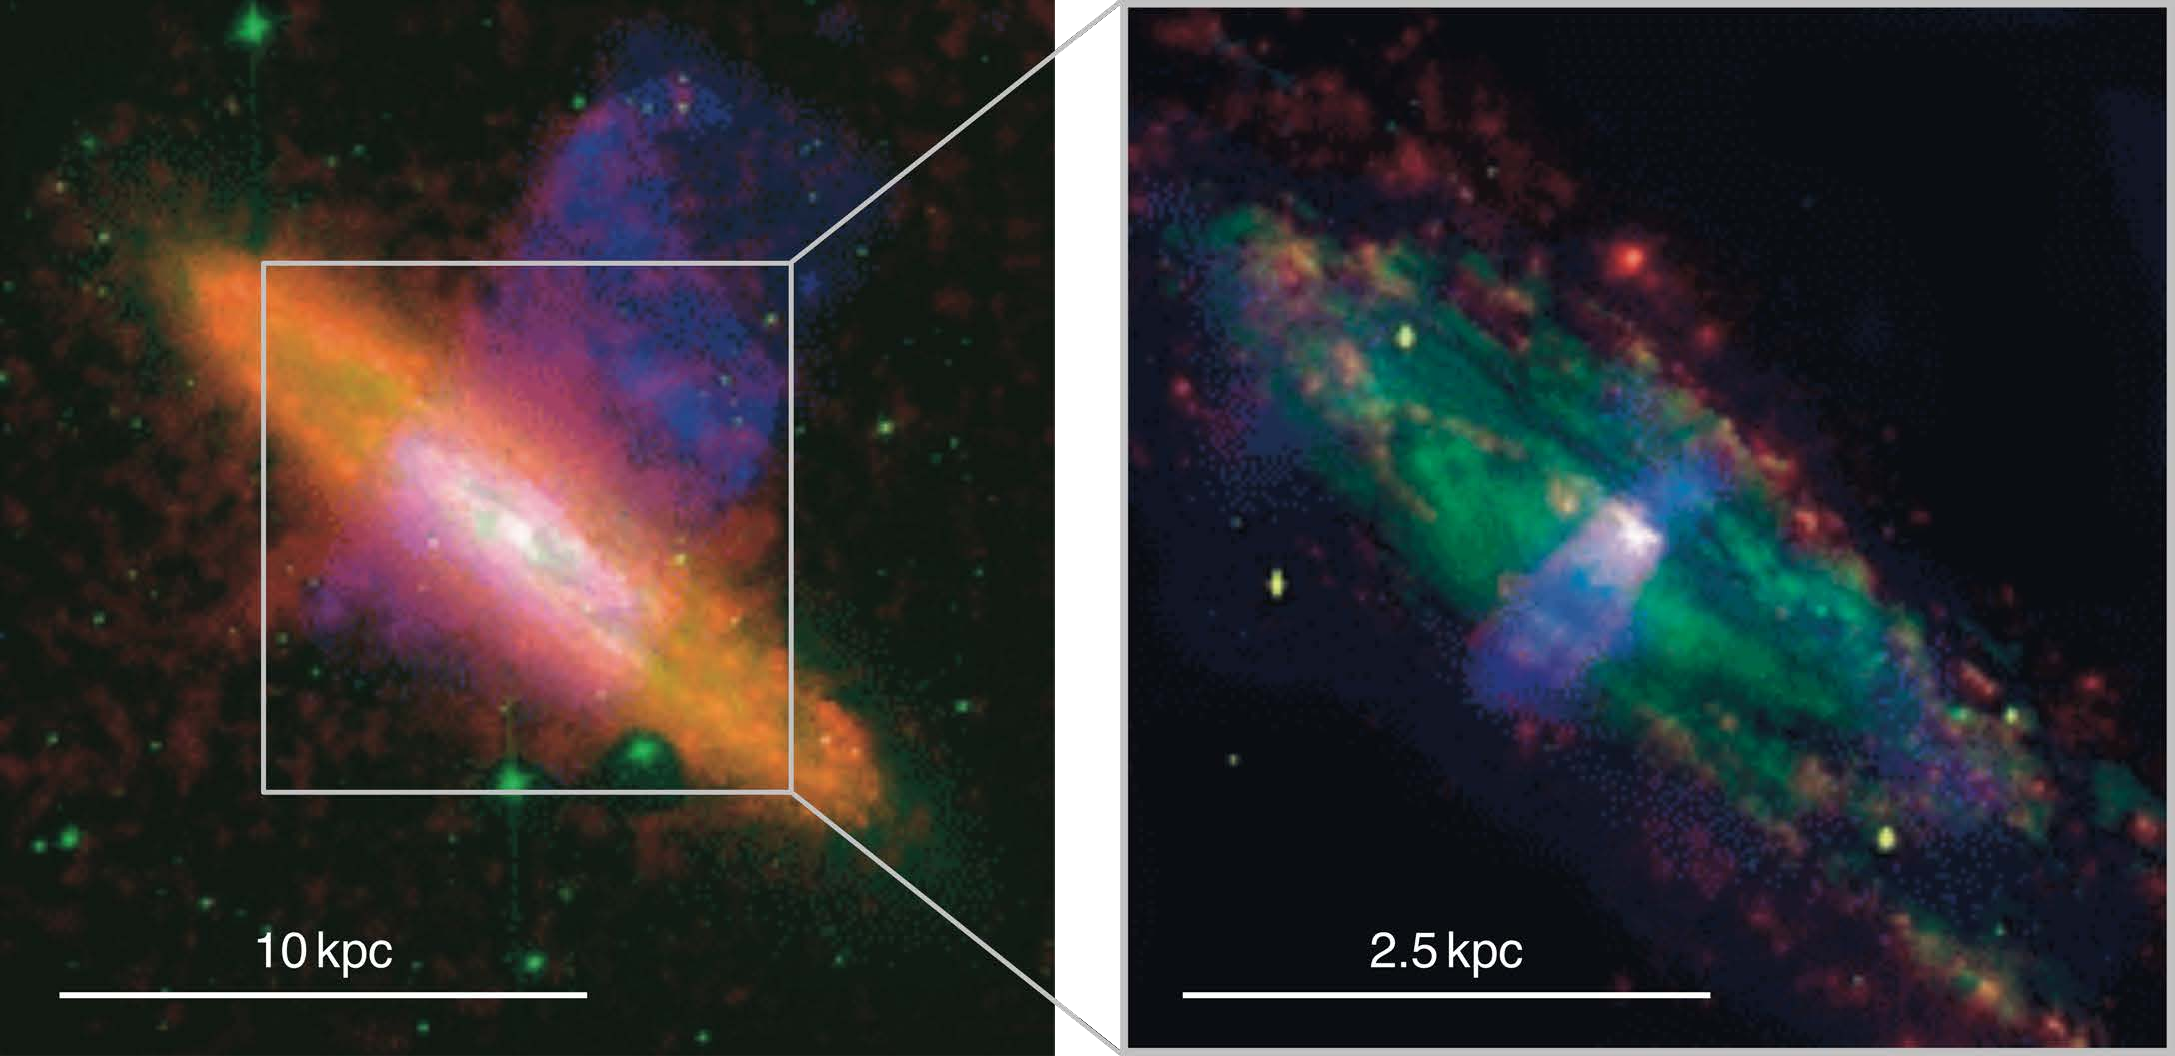
\includegraphics[width=\linewidth]{images/chapters/introduction/ngc253/Strickland+04_combined.pdf}
	\caption[Ionized outflow in \ngc253]{Three color composite image of \ngc253 showing \Halpha (red), optical R band (green) and soft X-ray ($0.3-2.0$\,keV, blue). Figure adopted from \citet{2004ApJ...606..829S}.}
	\label{introduction: figure: NGC253: Strickland}
\end{figure*}

Studies of the molecular gas phase in \ngc253 showed that its central starburst is fueled by gas accretion along the bar \citep{2004ApJ...611..835P}. The molecular ISM in the nuclear region is structured in several clumps that show high temperatures of $\GTRSIM 50$\,K \citep{2004ApJ...611..835P,Sakamoto:2011et,2019ApJ...871..170M}. 

From earlier low resolution observations \citep[$\GTR 20$\,pc, e.g.][]{2006ApJ...636..685S,Sakamoto:2011et} to recent observations at high resolution ($8\,\mathrm{pc}\times5$\,pc in \citealt{2017ApJ...849...81A} and 2\,pc in \citealt{2018ApJ...869..126L}) the number of molecular clumps associated with the starburst increased from $\sim5$ to 14. These studies find the clumps to be massive ($M_\mathrm{mol} \sim 4-10 \times 10^4$\,\Msun), compact ($\LESS 10$\,pc), chemically rich (up to $\GTR 19$ molecules detected in the 0.8\,mm band) and hot (up to 90\,K). 
These massive and dense clumps provide an ideal environment for SSC formation and each clump likely hosts an embedded massive (proto-)SSC \citep{2018ApJ...869..126L}.
It has been known for a while now that \ngc253 hosts at least a single SSC. \citet{Watson:1996dn} and \citet{Kornei:2009ee} detected a young, deeply embedded SSC in HST imaging of the nuclear region. Hints of further SSCs were discovered in radio observations \citep{1997ApJ...488..621U} but do not show obvious counterparts in optical or near-IR imaging \citep{2017ApJ...835..265W}. 
The 14 (proto-)SSCs characterized by \citet{2018ApJ...869..126L} are still deeply embedded in their natal gas and dust clouds. At least some of the SSCs are very young \citep[$\LESS 1$\,Myr][]{2020MNRAS.491.4573R}, with many showing roughly equal, but still uncertain, masses of young stars and gas \citep{2018ApJ...869..126L}.

Further structures in the molecular gas are shells and bubbles blown by stellar feedback. \citet{2006ApJ...636..685S} found two 100\,pc diameter superbubbles. \citet{2013Natur.499..450B} report molecular streamers\footnote{The term {\em streamer} here denotes structures with a high aspect ratio that are typically oriented roughly perpendicular to the disk and often show a velocity gradient.} originating from these shells with a lower limit to the outflow rate of $\dot{M} \sim 3-9$\,M$_\odot$\,yr$^{-1}$, about three times the star formation rate. This estimate was revisited by \citet{2018ApJ...867..111Z}, based on observations that show that the CO emission associated with the most prominent streamer is optically thick, increasing it to $25-50$\,\Msunyr. The impact of the outflows on the amount of mass lost from the molecular gas reservoir, and thus the lifetime of the starburst, is significant. 

